

The methodology with which I will be tackling the research question was partly touched upon in the introduction section, but in this section I will go into more detail describing the relevant satellite data that I will be using in the training of the classification model. 

I will justify the choice of a classification model trained with machine learning, detailing the specific machine learning algorithm, covering the benefits over other forms of autonomous data generation. 

The methodology in this project will closely follow those in similar studies using machine learning for classification models, such as \cite{ghansah_2022_monitoring}, meaning I will select a specific machine learning model upon which to train the classification model, clean the received results, and then deploy the algorithm over the intended land area. 

From these results, I will conduct data cleaning, which consists of correcting errors made in identifying water bodies. I expect the most likely causes of these errors will stem from difficulty in differentiating naturally occurring water bodies, like lakes and ponds, from man-made water reservoirs. To account for this, some previous models have used the satellite imagery metrics to eliminate identified water bodies below a certain defined surface area \citep{ghansah_2022_monitoring}. Another approach is to manually eliminate known, man-made water bodies that may be water reservoirs but do not fit in the selection criteria because they are not reservoirs for farm use (e.g. dams or outdoor pools). 

The initial plan of implementation for the model is to first train it on hand-selected images that contain water reservoirs that should be clearly identified, some that may be confused for other bodies of water, and pieces of land that may resemble water reservoirs due to their shape and size. Then the results will be cleaned as described above, and once the model has reached a satisfactory level of classification accuracy, the next step is to then deploy the algorithm for scanning over larger land areas covering much of east England. 

\section{Objective 1: Image Selection}
\subsection{Satellite Choice}
The satellite of choice for this thesis is Sentinel 2 because of the higher resolution options compared to Landsat 7-9. Additionally, for low-computation troubleshooting, the Sentinel 2 image folders also have a 60m resolution option, reducing time spent on opening and handling the otherwise larger image arrays. 

\subsection{Satellite Compatibility}
While the KRISP trainer program was developed primarily with Sentinel 2 in mind, it is entirely sensor-agnostic, meaning that dependent on specifically Sentinel 2 data. The KRISP trainer program is not only sensor-agnostic, but also 

The NALIRA program was initially developed for Landsat 7 images, then it was adapted for compatibility with any processing level of Landsat 8 and 9 as well. Then, Sentinel 2 data was introduced, and there was a brief period where NALIRA was capable of accepting any image from Landsat 7, Landsat 8, Landsat 9, Sentinel 2A, Sentinel 2B, and Sentinel 2C. 

\subsection{Image Download}


\section{IPDMP System Overview}
The Individual Project Data-to-Model Pipeline (IPDMP) comprises three core Python scripts designed for the classification of small water reservoirs using Sentinel-2 satellite imagery. The overall process involves data generation and labelling (NALIRA), model training (KRISP trainer), and model deployment for prediction (KRISP).

For this study, the Normalised Difference Water Index (NDWI) is selected as the primary spectral index for data labelling and model training/validation due to its ability to leverage Sentinel-2's high-resolution bands (Green and NIR). While other indices like MNDWI, AWEI-SH, and AWEI-NSH are calculated in NALIRA to aid manual labelling by providing multiple visual inputs, the machine learning model focuses on NDWI-derived data.

\begin{lstlisting}[language=Python, caption=Calculation of Water Detection Indices]
np.seterr(divide="ignore", invalid="ignore")
ndwi = ((green - nir) / (green + nir))
mndwi = ((green - swir1) / (green + swir1))
awei_sh = (green + 2.5 * blue - 1.5 * (nir + swir1) - 0.25 * swir2)
awei_nsh = (4 * (green - swir1) - (0.25 * nir + 2.75 * swir2))
\end{lstlisting}

Cloud masking employs a basic numerical threshold approach. Pixels in the Sentinel-2 cloud probability band (\verb|MSK_CLDPRB|) with a likelihood greater than 50\% are masked (set to NaN or zero) in the band images before index calculation. This simple method is deemed sufficient due to the selection of imagery from a period with known low cloud cover (March 2025). For applications in cloudier periods, more advanced masking techniques (e.g., FMask) and image compositing would be necessary.

A custom Keras-based Convolutional Neural Network (CNN) model, adapted from a TensorFlow tutorial, is used for classification. This approach offers flexibility and aims for good generalisation on the study area. The model is trained to classify image segments into 'reservoirs', 'water bodies' (non-reservoir), or 'land'. The KRISP script then deploys this trained model, applying it iteratively across small image chunks ('mini-chunks') derived from the larger satellite scene, effectively acting as an object detection mechanism for water reservoirs.

\section{Objective 2: Data Generation (NALIRA)}
NALIRA is responsible for processing raw Sentinel-2 imagery, calculating water indices, and facilitating the manual labelling process to create the training dataset for the Keras model.

\subsection{NALIRA Code Walk-through}

\subsubsection{Preliminaries}
This initial phase involves importing necessary libraries (os, numpy, csv, PIL, time, custom modules like \verb|data_handling|, \verb|image_handling|, misc, \verb|user_interfacing|), defining global constants and settings (DPI for plots, number of chunks, resolution choice, plotting/saving flags, data filename), and setting up the home directory path based on the operating environment (personal PC vs. university machine). It also records the start time for performance tracking.

\subsubsection{Initial Image Handling}
This section focuses on locating and loading the required Sentinel-2 spectral band image files.
\textbf{File Paths}
It constructs the full paths to the necessary band image files (.jp2 format) based on the satellite name, number, specific image folder name, and the chosen resolution ('10m' or '60m'). It handles Sentinel-2's specific folder structure, including navigating the 'GRANULE' subdirectories and selecting the appropriate resolution folders ('R10m', 'R20m', 'R60m'). It uses helper functions (\verb|get_sentinel_bands|) to determine the correct band identifiers (e.g., 'B03' for Green, 'B08' for NIR at 10m). For high-resolution processing, it combines paths from both R10m and R20m folders as needed (e.g., SWIR bands are only available at 20m).
\textbf{Converting Image to Array}
Converting Image to Array: The \verb|image_to_array| function (from \verb|image_handling.py|) is used to open each specified band image file and convert its pixel data into a NumPy array. For high-resolution mode where bands have different native resolutions (10m and 20m), lower-resolution arrays (20m SWIR1, SWIR2) are upscaled later during cloud masking using \verb|upscale_image_array| to match the 10m resolution arrays before index calculation. The resulting arrays are stored in a list.

\subsubsection{Cloud Masking}
This step aims to remove cloud-contaminated pixels from the band image arrays. It uses the Sentinel 2 Cloud Probability mask file (\verb|MSK_CLDPRB_20m.jp2| or \verb|MSK_CLDPRB_60m.jp2|). 
\begin{itemize}
    \item The appropriate resolution cloud mask file is opened and converted to a NumPy array using \verb|image_to_array|.
    \item If high-resolution bands are used, the 20m cloud mask is upscaled by a factor of 2 (\verb|upscale_image_array|) to match the 10m band resolution. The 20m SWIR1 and SWIR2 band arrays are also upscaled here.
    \item Pixels in the cloud mask array with a probability value greater than 50 are set to 100.
    \item The coordinates (indices) of these high-probability cloud pixels are identified using \verb|np.argwhere|.
    \item These coordinates are then used to set the corresponding pixel values in all the loaded band image arrays (Blue, Green, NIR, SWIR1, SWIR2) to 0, effectively masking them out before index calculation.
\end{itemize}

\subsubsection{Calculating Water Indices}
With the cloud-masked (and potentially upscaled) band arrays ready, this section calculates various water indices.
\begin{itemize}
    \item The NumPy arrays, initially of type \verb|uint16|, are converted to integer type (\verb|astype(int)|) to prevent overflow issues during calculations.
    \item The required bands are unpacked: Blue, Green, NIR, SWIR1, SWIR2.
    \item NumPy's error settings are adjusted to ignore division by zero and invalid value errors that can occur during index calculation (e.g., division by zero if both bands are zero).
    \item All four indices discussed in the methodology (NDWI, MNDWI, AWEI-SH, and AWEI-NSH) are calculated pixel-wise using standard formulas. 
    \item The resulting index arrays (NDWI, MNDWI, AWEI-SH, AWEI-NSH) are stored in a list.
\end{itemize}

\subsubsection{Note on Varying Resolutions}
The images generated by combining 10m and 20m resolution data can appear to have a slightly higher effective resolution than pure 20m images due to the way these indices are calculated. For indices requiring bands of different native resolutions—such as MNDWI, AWEI-SH, and AWEI-NSH—the lower resolution 20m bands (like SWIR1, SWIR2, and the 20m cloud mask) are upscaled to match the 10m resolution of bands such as Blue, Green, and NIR. During this process, each pixel from the 20m image effectively becomes four pixels, as both the height and width are doubled, ensuring that pixel-wise operations are compatible before performing the index calculations (see step 3.3.3).

% !!!!! PLACEHOLDER !!!!!
\begin{figure}[ht]
    \centering
    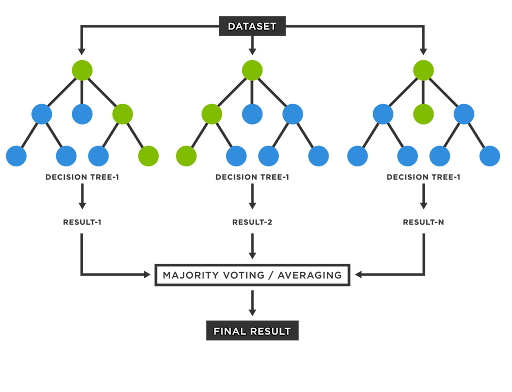
\includegraphics[width=0.6\textwidth]{contents/figures/LR RF diagram.jpg}
    \caption{SVM Confusion Matrix \citep{maity_2016}}
    \label{fig:NOTHING}
\end{figure}
% !!!!! PLACEHOLDER !!!!!

This means that for the calculation of MNDWI, for example, although four pixels of SWIR1 will all have the same value (because they have effectively been 'quadruplicated' to fit the same size array) the four pixels of Green will have the same resolution they had before, meaning they may change slightly from pixel to pixel. This has the effect of creating 2x2 pixel boxes of similar colours because only one of the two bands are changing in value, while the other stays stagnant, effectively limiting the maximum range of change within these boxes. 

\subsubsection{Displaying Indices}
This optional step visualizes the calculated water index arrays using Matplotlib.
\begin{itemize}
    \item It checks the \verb|show_index_plots| flag. If \verb|False|, the step is skipped.
    \item If \verb|True|, it iterates through the calculated index arrays (NDWI, MNDWI, AWEI-SH, AWEI-NSH).
    \item For each index, it creates a \verb|matplotlib| figure (\verb|plt.figure|) and displays the index array as an image (\verb|plt.imshow|).
    \item A title indicating the satellite, index name, DPI, and resolution is added. Axis labels and ticks are hidden for clarity.
    \item It checks the \verb|save_images| flag. If \verb|True|, the plot is saved as a PNG file (\verb|plt.savefig|) with a descriptive name, handling potential duplicate filenames by appending a counter.
    \item The plot is displayed on the screen ('plt.show').
\end{itemize}

\subsubsection{Data File Preparation}
This section prepares the CSV file used to store the manual labels.
\begin{itemize}
    \item It defines the path for the labelling data, creating the 'training data' subdirectory if it doesn't exist using \verb|change_to_folder|.
    \item The target CSV filename (\verb|responses_<n_chunks>_chunks.csv|) is defined.
    \item \verb|blank_entry_check| is called to remove any empty rows from the CSV file, ensuring data integrity. \verb|check_file_permission| is called within \verb|blank_entry_check| to avoid errors if the file is open elsewhere.
    \item File Validity Check: The script reads the existing CSV file (if any) and checks for validity. It verifies that the first column (chunk number) increments sequentially. If inconsistencies (e.g., missing chunks, incorrect order) or formatting errors are found, it prompts the user to retry, create a new file ('new'), or quit ('quit'). If a new file is created, it writes the header row and a dummy first entry.
    \item Data Completion Check: After validating the sequence, it checks if existing entries are complete. It iterates through the rows, verifying that if a row indicates the presence of reservoirs (column 1 \textgreater 0) or water bodies (column 2 \textgreater 0), the corresponding coordinate columns (column 3 onwards for reservoirs, column 8 onwards for bodies) actually contain coordinate data (identified by starting with '['). It also flags rows where coordinates exist but the count is zero. If incomplete or inconsistent rows are found, it sets a \verb|data_correction| flag and identifies the row indices needing correction. The labelling process (Step 6) will start from the first problematic chunk if \verb|data_correction| is \verb|True|.
    \item The starting chunk index \verb|i| is set to the last valid chunk number + 1, or to the index of the first invalid chunk if \verb|data_correction| is \verb|True|.
\end{itemize}

\textbf{Data File Format}
\begin{table}[h]
\centering
\begin{tabular}{l | l | l | l | l}
Chunk & Reservoirs & Water Bodies & Reservoir Positions & Water Body Positions \\
\hline
0 & 0 & 0 & - & - \\
1 & 1 & 0 & 12 11 31 33 & - \\
2 & 0 & 1 & - & 12 11 31 33 \\
3 & 1 & 1 & 12 11 31 33 & 12 11 31 33 \\
i & (n res) & (n bodies) & ulx uly lrx lry & ulx uly lrx lry \\
\end{tabular}
\caption{Example data file entries}
\label{tab:abc}
\end{table}

\subsubsection{Manual Data Labelling}
This interactive step uses a Tkinter GUI for the user to label reservoirs and other water bodies within image chunks. It only runs if the \verb|label_data| flag is \verb|True|.
\begin{itemize}
    \item It iterates through the image chunks, starting from the index \verb|i| determined in the previous step.
    \item For each chunk \verb|i|:
        \begin{itemize}
            \item \verb|plot_chunks| displays the NDWI, MNDWI, and TCI (True Color Image) representations of the current chunk, along with a low-resolution overview TCI showing the chunk's location. Maximum NDWI and MNDWI values for the chunk are printed.
            \item The user is prompted in the console to enter the number of reservoirs and non-reservoir water bodies visible in the chunk.
            \item \textbf{Input Handling:} The code handles integer inputs for counts. It also accepts \texttt{"break"} (to save progress and exit), \texttt{"back"} (to go back and re-label the previous chunk(s) by removing entries from the CSV), or \texttt{"back n"} (to go back n chunks). Error handling catches non-integer inputs.
            \item \textbf{ROI Selection:} If the user enters a non-zero count for reservoirs or water bodies, the \verb|prompt_roi| function is called. This function displays the TCI chunk in a Tkinter window. The user draws bounding boxes around the specified number of features. \verb|prompt_roi| returns a list of coordinates (\([ulx, uly, lrx, lry]\)) for each drawn box. These coordinates are appended to the \verb|entry_list| for the current chunk.
            \item \textbf{Saving Results:} After gathering counts and coordinates for a chunk, the \verb|entry_list| (containing chunk index, reservoir count, body count, reservoir coordinates\ldots, body coordinates\ldots) is formatted into a comma-separated string.
                \begin{itemize}
                    \item If in \verb|data_correction| mode, the existing line in the \verb|lines| list (read from the CSV earlier) is overwritten with the new data, and the entire file is rewritten. The index \verb|i| is then updated to the next invalid chunk index or proceeds normally if all corrections are done.
                    \item If not in \verb|data_correction| mode, the formatted string is appended as a new line to the \verb|data_file| CSV.
                \end{itemize}
            \item The loop continues until all chunks are processed or the user enters \verb|"break"|.
        \end{itemize}
\end{itemize}

\subsubsection{Data Segmentation}
After labelling is complete (or skipped), this step extracts the labelled regions (reservoirs and water bodies) and saves them as individual image files, thereby creating the dataset for the model trainer.
\begin{itemize}
    \item \textbf{Extract Coordinates:}
    \begin{itemize}
        \item It reads the completed \verb|data_file| CSV. It iterates through the rows, identifying chunks containing reservoirs (column 1 \> 0) and water bodies (column 2 \> 0). For each identified feature, it extracts the corresponding coordinates using \verb|extract_coords| and stores them along with the chunk number (e.g., \texttt{res\_coords = [(chunk\_num, [ulx, uly, lrx, lry]), \ldots]}). Sea areas identified by specific coordinates are excluded from the water body list.
        \item \textbf{Isolate and Save Images:} It iterates through the extracted reservoir coordinates (\verb|res_coords|) and water body coordinates (\verb|body_coords|).
        \begin{itemize}
            \item For each coordinate set:
            \begin{itemize}
                \item It determines the corresponding chunk number.
                \item It defines paths to save the segmented images (e.g., \texttt{training data/ndwi/reservoirs/}, \texttt{training data/tci/water bodies/}), creating directories if necessary using \verb|change_to_folder|.
                \item It calls \verb|save_image_file| once for the NDWI chunk (\verb|index_chunks[0]|), saving a normalized (\verb|colormap| applied based on global NDWI min/max multiplied by a factor) PNG image of the region defined by the coordinates plus a margin. The filename includes the chunk number and feature type/index (e.g., \verb|ndwi chunk 10 reservoir 1.png|). Duplicate checks prevent overwriting existing files. 
                \item Then calls \verb|save_image_file| once for the TCI chunk (\verb|tci_chunks|), saving a non-normalized PNG image of the same region plus a margin, with a similar filename structure (e.g., \verb|tci chunk 10 reservoir 1.png|).
            \end{itemize}
        \end{itemize}
        \item \textbf{!!! ADD SECTION ON SAVING "NEITHER" CHUNKS !!!}
    \end{itemize}
\end{itemize}

\section{Objective 3: Model Training (KRISP Trainer)}
This script trains the Keras CNN model using the segmented image data generated by NALIRA.

\subsection{KRISP Trainer Code Walk-through}

\subsubsection{Preliminaries}
Imports necessary libraries: \verb|time|, \verb|pathlib|, \verb|os|, \verb|matplotlib|, \verb|numpy|, \verb|datetime|, \verb|sys|, \verb|tensorflow|, \verb|keras|. It also imports \verb|image_to_array| and spinner functions from custom modules. Records the \verb|MAIN_START_TIME|.

\subsubsection{Path Handling}
Defines and validates paths used throughout the script:
\begin{itemize}
    \item \verb|BASE_PROJECT_DIR|: Root directory of the project.
    \item \verb|SENTINEL_FOLDER|: Specific Sentinel-2 image folder being used.
    \item \verb|DATA_BASE_PATH|: Path to the training data directory created by NALIRA.
    \item \verb|DATA_DIR_NAME|: Specifies the subdirectory containing the images to train on (\texttt{ndwi} or \texttt{tci}).
    \item \verb|MODEL_SAVE_DIR|: Directory where the trained model will be saved.
    \item \verb|MODEL_FILENAME|: Name for the saved model file (includes type and epoch count).
    \item \verb|TEST_IMAGE_SUBDIR| and \verb|TEST_IMAGE_NAME|: Path components for a sample image used for a final prediction test.
    \item It constructs the full paths (\verb|data_dir|, \verb|model_save_path|, \verb|test_image_path|).
    \item It checks if the \verb|data_dir| exists; if not, it prints an error and exits.
    \item It checks if the \verb|test_image_path| exists and prints a warning if not.
    \item It creates the \verb|MODEL_SAVE_DIR| if it doesn't exist and \verb|SAVE_MODEL| is \verb|True|.
    \item It counts the number of PNG images within the class subdirectories (\verb|reservoirs|, \verb|water bodies|) inside \verb|data_dir| using \verb|pathlib| and prints the count, warning if it's zero or less than the batch size.
\end{itemize}

\subsubsection{Dataset Preparation}
Loads and prepares the image dataset for training and validation using TensorFlow/Keras utilities.
\begin{itemize}
    \item \verb|tf.keras.utils.image_dataset_from_directory|: This function loads images from the specified \verb|data_dir|. It automatically infers class labels (\verb|reservoirs|, \verb|water bodies|) from the subdirectory names.
    \begin{itemize}
        \item \verb|validation_split|: Reserves a fraction of the data for validation (e.g., 0.2 for 20\%).
        \item \verb|subset|: Specifies \verb|training| or \verb|validation| to get the respective datasets.
        \item \verb|seed|: Ensures the split is reproducible.
        \item \verb|image_size|: Resizes all images to the specified height and width (e.g., 157x157).
        \item \verb|batch_size|: Groups images into batches (e.g., 32).
    \end{itemize}
    \item It retrieves the \verb|class_names| from the loaded dataset and checks that there are at least two classes.
    \item Performance Optimization:
    \begin{itemize}
        \item \verb|AUTOTUNE|: Lets TensorFlow dynamically tune prefetching buffer sizes.
        \item \verb|.cache()|: Caches the datasets in memory (after the first epoch) for faster subsequent access.
        \item \verb|.shuffle()|: Randomly shuffles the training dataset (buffer size determines the extent of shuffling).
        \item \verb|.prefetch()|: Prepares subsequent batches while the current batch is being processed by the model, overlapping data loading/preprocessing with training steps.
    \end{itemize}
\end{itemize}


\subsubsection{Model Improvements}
Defines strategies to improve model performance and prevent overfitting, common with smaller datasets.

\textbf{Data Augmentation}
A \verb|keras.Sequential| layer named \verb|data_augmentation| is defined. It includes:
\begin{itemize}
    \item \verb|layers.RandomFlip("horizontal")|: Randomly flips images horizontally.
    \item \verb|layers.RandomRotation(0.1)|: Randomly rotates images by a small fraction.
    \item \verb|layers.RandomZoom(0.1)|: Randomly zooms into images.
    \item This layer will be added as the first layer of the main model, applying these transformations on-the-fly during training to increase dataset diversity. The \verb|input_shape| is specified here.
\end{itemize}

\textbf{Dropout}
A \verb|layers.Dropout(DROPOUT_RATE)| layer is included in the main model architecture (defined later). During training, it randomly sets a fraction (\verb|DROPOUT_RATE|, e.g., 0.2) of input units to 0 at each update step, which helps prevent overfitting by reducing reliance on specific neurons. The CNN model itself is defined as a \verb|keras.Sequential| model:
\begin{itemize}
    \item \textbf{Input:} Data Augmentation layer, followed by \verb|layers.Rescaling(1./255)| to normalise pixel values from [0, 255] to [0, 1].
    \item \textbf{Convolutional Blocks:} Three blocks, each consisting of:
    \begin{itemize}
        \item \verb|layers.Conv2D|: Learns spatial hierarchies of features (16, 32, 64 filters, 3x3 kernel, \verb|"same"| padding, \verb|ReLU| activation).
        \item \verb|layers.MaxPooling2D|: Downsamples the feature maps, reducing dimensionality and providing spatial invariance.
    \end{itemize}
    \item \textbf{Dropout Layer:} Applied after the convolutional blocks.
    \item \texttt{layers.Flatten}: Converts the 2D feature maps into a 1D vector.
    \item \texttt{layers.Dense(128, activation='relu')}: A fully connected hidden layer.
    \item \textbf{Output Layer:} \verb|layers.Dense(num_classes)|: The final output layer with units equal to the number of classes. It outputs raw \verb|logits| (no activation function here, as specified by \verb|from_logits=True| in the loss function).
\end{itemize}
The model is compiled using \verb|model.compile()|:
\begin{itemize}
    \item \texttt{optimizer}: Adam optimizer with a specified \verb|LEARNING_RATE|.
    \item \texttt{loss}: \verb|tf.keras.losses.SparseCategoricalCrossentropy(from_logits=True)| is used because the labels are integers (0, 1, ...) and the model outputs \verb|logits|.
    \item \verb|metrics|: Tracks \verb|accuracy| during training and evaluation.
\end{itemize}

\subsubsection{Model Training}
Executes the training process.
\begin{itemize}
    \item \verb|model.fit()|: This function trains the model.
    \begin{itemize}
        \item \verb|train_ds|: The prepared training dataset.
        \item \verb|validation_data=val_ds|: The prepared validation dataset, used to evaluate performance on unseen data after each epoch.
        \item \verb|epochs=EPOCHS|: The number of times the entire training dataset is passed through the model.
    \end{itemize}
    \item The training history (accuracy, loss, validation accuracy, validation loss for each epoch) is stored in the \verb|history| object. Error handling wraps the \verb|fit| call.
\end{itemize}

\subsubsection{Training Result Visualisation}
Plots the training and validation accuracy and loss curves over epochs using \verb|matplotlib|.
\begin{itemize}
    \item It checks if the \texttt{history} object exists (i.e., if training completed successfully).
    \item Extracts accuracy (\texttt{acc}), validation accuracy (\verb|val_acc|), loss (\texttt{loss}), and validation loss (\verb|val_loss|) from \texttt{history.history}.
    \item Creates a figure with two subplots:
    \begin{itemize}
        \item Left subplot: Plots training vs. validation accuracy against epochs.
        \item Right subplot: Plots training vs. validation loss against epochs.
    \end{itemize}
    \item Adds labels, titles, legends, and adjusts axis limits for clarity.
    \item \verb|plt.tight_layout()| adjusts spacing, and \texttt{plt.show()} displays the plots.
\end{itemize}

\subsubsection{Predicting on New Data}
Uses the trained model to predict the class of a single, predefined test image.
\begin{itemize}
    \item Checks if the \verb|test_image_path| exists.
    \item Loads the test image using \verb|image_to_array| and displays it using \texttt{plt.imshow}.
    \item Loads the same image using \verb|tf.keras.utils.load_img|, resizing it to the model's expected input size (\verb|IMG_HEIGHT|, \verb|IMG_WIDTH|).
    \item Converts the image to a NumPy array (\verb|img_to_array|) and adds a batch dimension (\verb|tf.expand_dims|).
    \item \verb|model.predict()|: Feeds the prepared image array to the trained model to get predictions (\verb|logits|).
    \item \texttt{tf.nn.softmax()}: Converts the output logits into probabilities for each class.
    \item \texttt{np.argmax()}: Finds the index of the class with the highest probability.
    \item Retrieves the corresponding \verb|class_name| using the index.
    \item Calculates the confidence percentage (\texttt{100 * np.max(score)}).
    \item Prints the predicted class name and confidence score. It also includes a simple check to see if the prediction matches the expected class based on the filename (\texttt{"reservoir"}).
\end{itemize}

\subsubsection{Saving and Summary}
Optionally saves the trained model and prints a final summary.
\begin{itemize}
    \item Checks the '\verb|SAVE_MODEL|' flag and if training was successful ('history' exists).
    \item If the target '\verb|model_save_path|' already exists, it creates a new versioned filename by appending a timestamp ('\verb|_YYYYMMDD_HHMMSS|') to avoid overwriting.
    \item '\verb|model.save()|': Saves the entire model (architecture, weights, optimizer state) to the specified path in Keras format ('\verb|.keras|').
    \item Prints the final save path or error messages if saving fails.
    \item Prints the total script execution time.
\end{itemize}

\section{Objective 4: Model Deployment (KRISP)}
This script deploys the trained Keras model (saved by \verb|KRISP_trainer|) to classify mini-chunks generated from a larger Sentinel-2 scene.

\subsection{KRISP Walk-through}

\subsubsection{Preliminaries}
Imports necessary libraries: time, os, numpy, sys, re (for regex filename parsing), math, matplotlib, tensorflow, keras. Imports custom functions: '\verb|image_to_array|', '\verb|mask_sentinel|', '\verb|save_image_file|', '\verb|split_array|', '\verb|create_9_random_coords|', spinner functions. Sets up the home directory path. Defines '\verb|class_names|'.

\subsubsection{Checking for Pre-Existing Files}
This section manages the generation of small image 'mini-chunks' from the input Sentinel-2 scene, which will be fed into the model for prediction. It includes checks to avoid regenerating data unnecessarily.
\begin{itemize}
    \item Defines the path ('\verb|test_data_path|') where the NDWI mini-chunk images will be saved (e.g., '\verb|test data/ndwi_0.4/|').
    \item Lists existing files in that directory.
    \item Uses \verb|regex| ('\verb|re.compile|') to parse filenames like '\verb|ndwi chunk <i> minichunk <j>.png|' to find the highest chunk index ('\verb|max_chunk_index|') already processed and saved.
    \item Calculates remaining chunks and percentage.
    \item If existing chunks are found, it prompts the user ('input()') whether to continue generating the remaining chunks ('\verb|generate_chunks = True|') or exit ('\verb|sys.exit(0)|'). If no existing files match or the directory doesn't exist, it assumes generation is needed ('\verb|generate_chunks = True|' implicitly or explicitly).
\end{itemize}

\subsubsection{Initial Image Handling (Conditional)}
Note: this step only runs if \verb|generate_chunks| is \verb|True|.

\begin{itemize}
    \item Locates and opens the Green (B03) and NIR (B08) 10m band images from the specified Sentinel-2 folder, similar to NALIRA (steps 3.3.2).
    \item Converts them to NumPy arrays using '\verb|image_to_array|'.
\end{itemize}

\subsubsection{Cloud Masking (Conditional)}
Note: this step only runs if \verb|generate_chunks| is \verb|True|.

\begin{itemize}
    \item Applies cloud masking using the 20m cloud probability file, upscaling the mask to 10m resolution, similar to NALIRA (step 3.3.3). The function '\verb|mask_sentinel|' modifies the '\verb|image_arrays|' (Green, NIR) in place.
\end{itemize}

\subsubsection{Calculating NDWI (Condtional)}
Note: this step only runs if \verb|generate_chunks| is \verb|True|.

Calculates the NDWI array from the masked Green and NIR arrays, similar to NALIRA (step 3.3.4).

\subsubsection{True Colour Image Handling (Optional)}
Note: this step only runs if \verb|generate_chunks| is \verb|True|. 

\subsubsection{Generating Chunks and Saving Images (Conditional)}
Note: this step only runs if \verb|generate_chunks| is \verb|True|.

\begin{itemize}
    \item Splits the full NDWI array into '\verb|n_chunks|' using '\verb|split_array|'.
    \item Determines the global minimum and maximum NDWI values across all chunks (max is scaled by '\verb|max_multiplier|').
    \item Iterates through the NDWI chunks ('\verb|ndwi_chunks|'). If resuming, it skips chunks with index less than '\verb|start_chunk_index|'.
    \item For each chunk '\verb|i|':
    \begin{itemize}
        \item '\verb|create_9_random_coords|': Generates coordinates for 9 slightly overlapping mini-chunks within the current chunk.
        \item For each mini-chunk coordinate set 'j':
        \begin{itemize}
            \item Defines the output image name (e.g., 'ndwi chunk i minichunk j.png').
            \item '\verb|save_image_file|': Saves the mini-chunk region from the parent NDWI chunk 'i' as a normalised PNG image file in the '\verb|test_data_path|'. Normalization uses the pre-calculated global min/max. '\verb|dupe_check|' is \verb|False| as overwriting might be intended if resuming.
        \end{itemize}
    \end{itemize}
\end{itemize}


\subsubsection{Model Deployment}
Loads the pre-trained model and uses it to classify the generated (or pre-existing) NDWI mini-chunk images.
\begin{itemize}
    \item Load model
    \begin{itemize}
        \item Defines the path to the saved Keras model file ('\verb|model_path|') based on 'HOME', 'IPDMP', '\verb|saved_models|', and the specified '\verb|model_name|'.
        \item '\verb|keras.models.load_model()|': Loads the trained model architecture and weights.
    \end{itemize}
    \item Prediction Loop
    \begin{itemize}
        \item Gets a list of all mini-chunk image filenames from the '\verb|test_data_path|' (limited to the first 20 in the provided code for demonstration).
        \item Iterates through each '\verb|file_name|':
        \begin{itemize}
            \item Constructs the full '\verb|file_path|'.
            \item '\verb|tf.keras.utils.load_img()|': Loads the mini-chunk image, resizing it to the model's expected input dimensions ('height', 'width' - e.g., 157x157).
            \item Displays the loaded mini-chunk image using 'plt.imshow'.
            \item '\verb|tf.keras.utils.img_to_array()|': Converts the image to a NumPy array.
            \item '\verb|tf.expand_dims()|': Adds a batch dimension.
            \item 'model.predict()': Feeds the prepared image array to the loaded model, obtaining prediction logits.
            \item 'tf.nn.softmax()': Converts logits to class probabilities.
            \item 'np.argmax()': Finds the index of the highest probability class.
            \item Retrieves the corresponding '\verb|predicted_class_name|' from '\verb|class_names|'.
            \item Calculates the 'confidence' percentage.
            \item Prints the prediction result (class name and confidence) for the mini-chunk image.
        \end{itemize}
    \end{itemize}
\end{itemize}

\section{Technical Challenges}
\subsubsection{Identifying water}
One of the main challenges in this research will be the differentiation between water reservoirs from land areas, or other bodies of water. Below is a screenshot taken from Google Maps showing a farm in east England with a water reservoir on the left and some tree cover on the right. 

% !!! PLACEHOLDER !!!
\begin{figure}[H]
\centering
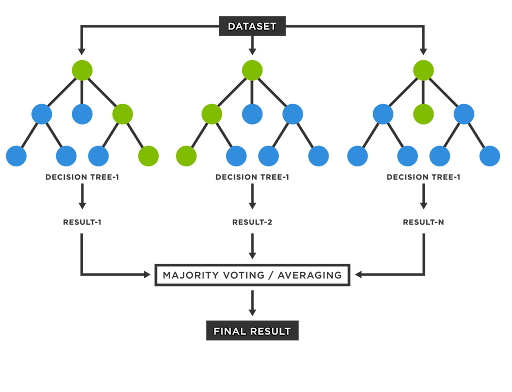
\includegraphics[width=0.4\textwidth]{contents/figures/LR RF diagram.jpg}
\caption{Google Maps screenshot showing a water reservoir near trees}
\label{fig:NISH}
\end{figure}
% !!! PLACEHOLDER !!!

In this example, a human could easily identify that the upper right side of this image shows trees, and the lower left side shows a river with a nearby water reservoir. However, a computer algorithm may find this differentiation more difficult, as relying solely on colours may lead it to the conclusion that both sides of the image contain a water reservoir. Instead, more complex techniques must be adopted that allow the computer to determine the shape, surrounding area, and other contextual information about the water reservoir. For this reason, one of the goals of this project is also to determine what the most valuable metrics are, from a satellite imagery perspective, for identifying water reservoirs. A further challenge will then be implementing these metrics and training a machine learning algorithm to make use of them to classify large areas of land. 

\subsubsection{Cloud Contamination}
Satellite imagery can come in many different levels of quality, and one of the main problems that have to be mitigated for is potential cloud cover. Clouds can partially or completely obscure important features on land or they can 'trick' a program into predicting a water feature instead of a cloud or the shadow of a cloud. As mentioned before, the time period for this study was specifically selected to avoid this problem entirely, however for the cases where clouds still cover part of the image, rudimentary cloud masking has been implemented, and will be discussed in further detail in upcoming sections. 

\subsubsection{Machine Learning Development}
There are also technical challenges that come with machine learning. Although resources for learning about this topic have improved in the past few years, there is still a steep learning gradient, particularly for one with little background in computer science. For this reason, the researcher has diligently documented progress on software development in this project with a public code repository which can be found linked in Appendix B. 

\section{Online Code Repository (GitHub)}
See appendix B
